%%
%% RQDQL.com
%%
%% This source file is subject to the new BSD license that is bundled
%% with this package in the file LICENSE.txt. It is also available
%% through the world-wide-web at this URL: http://www.rqdql.com/LICENSE.txt
%% If you did not receive a copy of the license and are unable to
%% obtain it through the world-wide-web, please send an email
%% to license@rqdql.com so we can send you a copy immediately.
%%
%% THIS SOFTWARE IS PROVIDED BY THE COPYRIGHT HOLDERS AND CONTRIBUTORS
%% "AS IS" AND ANY EXPRESS OR IMPLIED WARRANTIES, INCLUDING, BUT NOT
%% LIMITED TO, THE IMPLIED WARRANTIES OF MERCHANTABILITY AND FITNESS
%% FOR A PARTICULAR PURPOSE ARE DISCLAIMED. IN NO EVENT SHALL THE
%% COPYRIGHT OWNER OR CONTRIBUTORS BE LIABLE FOR ANY DIRECT, INDIRECT,
%% INCIDENTAL, SPECIAL, EXEMPLARY, OR CONSEQUENTIAL DAMAGES (INCLUDING,
%% BUT NOT LIMITED TO, PROCUREMENT OF SUBSTITUTE GOODS OR SERVICES; LOSS
%% OF USE, DATA, OR PROFITS; OR BUSINESS INTERRUPTION) HOWEVER CAUSED
%% AND ON ANY THEORY OF LIABILITY, WHETHER IN CONTRACT, STRICT LIABILITY,
%% OR TORT (INCLUDING NEGLIGENCE OR OTHERWISE) ARISING IN ANY WAY OUT
%% OF THE USE OF THIS SOFTWARE, EVEN IF ADVISED OF THE POSSIBILITY
%% OF SUCH DAMAGE.
%%
\documentclass{article}
\usepackage[T1]{fontenc} % to enable "{" symbol in \ttfamily
\usepackage{listings} % listings
    \lstset{
        basicstyle=\small\ttfamily,
        numbers=left,
        numberstyle=\scriptsize,
        firstnumber=1,
        stepnumber=4,
        numbersep=1em,
        aboveskip=2em,
        belowskip=1em,
        lineskip=-0.3em,
        frame=leftline,
    }
\usepackage{array} % complex TABULAR environments
\usepackage{color}
\usepackage[hyperfootnotes=true,unicode]{hyperref}
    \hypersetup{
        unicode=false,
        pdftoolbar=false,
        pdfmenubar=false,
        pdffitwindow=false,
        pdftitle={RQDQL White Paper},
        pdfauthor={RQDQL.com},
        pdfsubject={RQDQL White Paper},
        pdfnewwindow=true,
        colorlinks=true,
        linkcolor=blue,
        citecolor=blue,
        filecolor=blue,
        urlcolor=blue
    }
\usepackage[rgb]{xcolor}
    \definecolor{rupBody}{rgb}{1,1,0.8}
    \definecolor{rupBorder}{rgb}{0.6039,0,0.2}
\usepackage{tikz}
	\usetikzlibrary{shapes} % node split
	\usetikzlibrary{chains} % start chains
	\usetikzlibrary{arrows} % diamond
    \usetikzlibrary{decorations.pathmorphing}
    \usetikzlibrary{positioning}
    \usetikzlibrary{fit}
    \usetikzlibrary{trees} % for grow cyclic
    \tikzstyle{class} = [text ragged, font={\scriptsize\ttfamily}, fill=white, anchor=north,
        rectangle split, rectangle split parts=2,
        fill=rupBody, draw=rupBorder] % class in class diagram
    \tikzstyle{comment} = [font={\scriptsize\ttfamily}, fill=white] % comment in class diagram
    \tikzstyle{cardinality} = [font={\scriptsize\ttfamily}] % cardinality

\begin{document}
\setlength{\parindent}{0pt}
\setlength{\parskip}{1em}
\newcommand{\type}[1]{\mbox{\texttt{#1}}}
\newenvironment{maths}
{
    \vspace*{0.5em}
    \begin{tabular}{l>{\raggedright\arraybackslash}p{20em}}
}
{
    \end{tabular}
    \vspace*{1em}
}




\title{RQDQL: White Paper}
    \author{
        Yegor Bugayenko\\
        568 9th Str South, 202, \\
        Naples, FL 34102\\
        \texttt{yegor@rqdql.com}
    }
    \maketitle
    \begin{abstract}
        Requirements Definition and Query Language (RQDQL) is
        an experimental set of tools and formats that enables definition of
        an SRS document in a
        human-friendly language, and at the same time making it understandable
        by computers. Requirements in plain text are converted to
        second order logic predicates and then represented in MOF/XMI.
    \end{abstract}




\section{Introduction}

    IEEE 830 says: ``\emph{Software Requirements Specification should be
    correct, unambiguous, complete, consistent, ranked for importance and/or stability,
    verifiable, modifiable, traceable}''~\cite{ieee830}. RQDQL enables the creation
    of such documents in plain text format.

    First, we convert plain English into objects (in terms of object-oriented
    programming). Next, we convert objects into second order logic predicates.
    Then, we resolve predicates on data scope (in terms of logical programming)
    and create a collection of all possible scope variants. Then, for every
    scope variant we build a model in terms of MOF~\cite{mof2}, converting them later
    into XMI and transferring to the destination. Next, XMI~\cite{mof-to-xmi} can be rendered
    for an end-user or understood by a computer. Finally, the entire process
    is delivered to end-users in customizable XML~\cite{xml} reports.
    The workflow of the process explained is presented in Fig.~\ref{fig:Workflow}.

    \begin{figure}[ht]
        \caption{RQDQL highest-level workflow description, where we start
            from a plain English and finish with a strict formal description
            of a testing model, visible to end-user and a computer.}
        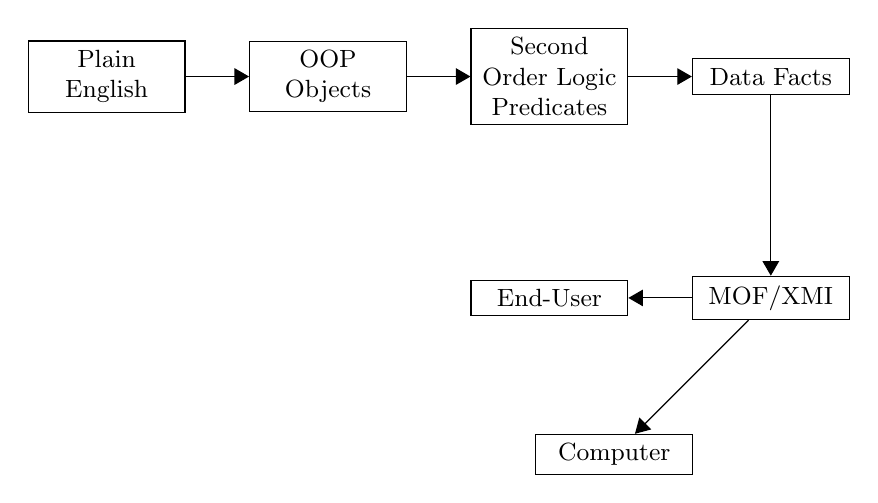
\begin{tikzpicture}[
            every node/.style={text width=5em, text centered, draw=black, font=\small},
            every path/.style={draw, -triangle 60},
            node distance=8em
        ]
            \node (english) {Plain English};
            \node [right of=english] (objects) {OOP Objects};
            \node [right of=objects] (sol) {Second Order Logic Predicates};
            \node [right of=sol] (data) {Data Facts};
            \node [below of=data] (mof) {MOF/XMI};
            \node [left of=mof] (user) {End-User};
            \node [below left of=mof] (computer) {Computer};
            \draw (english) -- (objects);
            \path (objects) -- (sol);
            \path (sol) -- (data);
            \path (data) -- (mof);
            \path (mof) -- (user);
            \path (mof) -- (computer);
        \end{tikzpicture}
        \label{fig:Workflow}
    \end{figure}

    Section~\ref{sec:to-objects} explains the process of converting plain English
    to ``object oriented thesaurus''. We are using
    \href{http://www.altlr.org}{\texttt{antlr3}} grammar analysis toolkit.
    Moreover, the entire RQDQL product is written in Java.

    Section~\ref{sec:to-solm} explains how objects are converted to
    second order logic ``predicates'',
    and validated. Here we also discuss the interconnection with
    Lisp~\cite{graham93}.

    Section~\ref{sec:to-data} explains the process of converting of
    second order predicates to Prolog-style data ``facts'', and reveals the internal
    structure of said facts. We discuss interconnection with Prolog~\cite{shapiro94}.

    Section~\ref{sec:front} is about an interface between \type{rqdql-bin.jar}
    command-line interface and its users.

    Section~\ref{sec:test-cases} explains the mechanism of conversion
    of data facts into test cases.

    Section~\ref{sec:design} contains the most important architecture
    and design decisions documented in diagrams.



\section{Plain English to Object Thesaurus}
\label{sec:to-objects}

    Detailed explanation of the RQDQL syntax is given on its
    website \href{http://www.rqdql.com}{www.rqdql.com}.

    In Java we use the following types:

    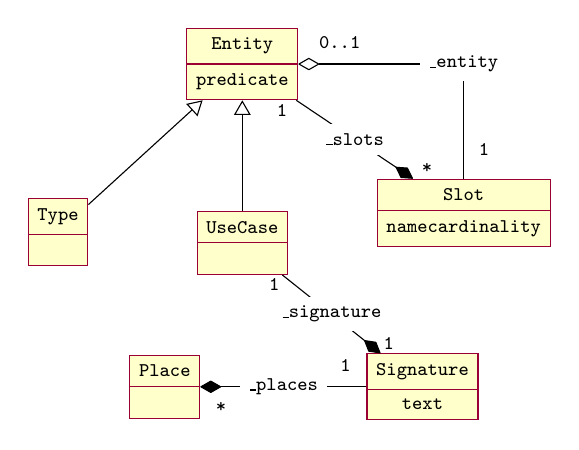
\begin{tikzpicture}
        \node [class] (entity) {Entity\nodepart{second}predicate};
        \node [class, below right=4em of entity] (slot) {Slot\nodepart{second}name\linebreak{}cardinality};
        \node [class, below left=5em of entity] (type) {Type\nodepart{second}};
        \node [class, below=4em of entity] (uc) {UseCase\nodepart{second}};
        \node [class, below right=4em of uc] (signature) {Signature\nodepart{second}text};
        \node [class, left=6em of signature] (place) {Place\nodepart{second}};
        \draw [-open triangle 60] (type) -- (entity);
        \draw [-open triangle 60] (uc) -- (entity);
        \draw [-diamond]
            (entity)
            --
            node [cardinality, very near start, left=0.5em] {1}
            node [comment] {\_slots} (slot)
            node [cardinality, very near end, right=0.5em] {*};
        \draw [-open diamond]
            (slot)
            |-
            node [cardinality, very near start, right=0.2em] {1}
            node [comment] {\_entity} (entity)
            node [cardinality, very near end, above=0.2em] {0..1};
        \draw [-diamond]
            (uc)
            --
            node [cardinality, very near start, left=0.2em] {1}
            node [comment] {\_signature} (signature)
            node [cardinality, very near end, right=0.2em] {1};
        \draw [-diamond]
            (signature)
            --
            node [cardinality, very near start, above=0.2em] {1}
            node [comment] {\_places} (place)
            node [cardinality, very near end, below=0.2em] {*};
    \end{tikzpicture}

    \subsection{Types}

        A simplified verbal form of a type looks like this:

    \begin{verbatim}
User includes:
  email: "email address";
  face-s: Photo "a collection of photos";
  manager: User "user's manager, if any";
  address.
Address of User includes: city, country.\end{verbatim}

        In Java the type is presented by class \texttt{Type} and
        the type written above will look like:

        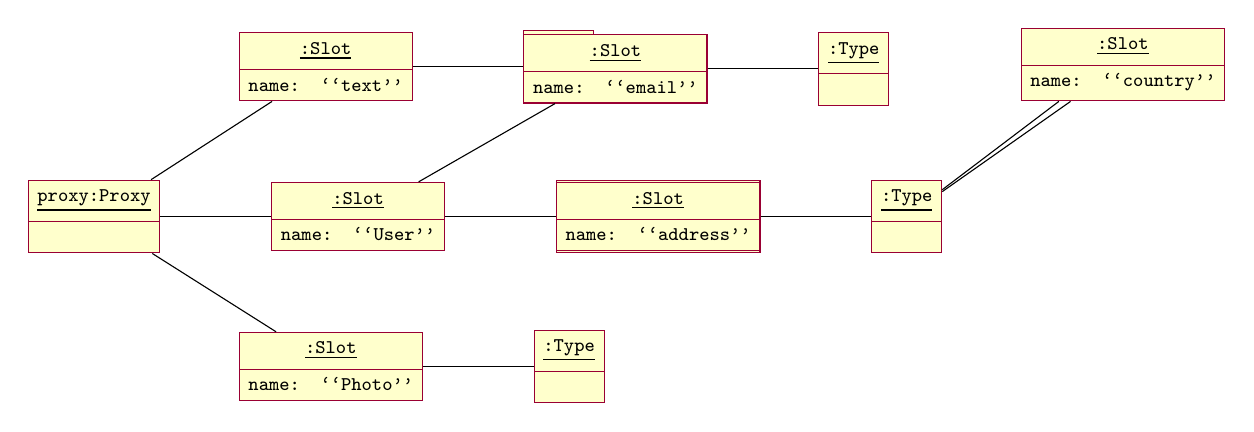
\begin{tikzpicture}[start chain, node distance=4em, every node/.style={on chain,join}, every join/.style={-}]
            \node [class, on chain] (proxy) {\underline{proxy:Proxy}\nodepart{second}};
            \begin{scope}[start branch=email]
                \node [class, on chain=going above right] {\underline{:Slot}\nodepart{second}name: ``text''};
                \node [class, on chain] {\underline{:Type}\nodepart{second}};
            \end{scope}
            \begin{scope}[start branch=user]
                \node [class, on chain] {\underline{:Slot}\nodepart{second}name: ``User''};
                \begin{scope}[start branch=email]
                    \node [class, on chain=going above right] {\underline{:Slot}\nodepart{second}name: ``email''};
                    \node [class, on chain] {\underline{:Type}\nodepart{second}};
                \end{scope}
                \begin{scope}[start branch=face]
                    \node [class, on chain] {\underline{:Slot}\nodepart{second}name: ``face''};
                \end{scope}
                \begin{scope}[start branch=manager]
                    \node [class, on chain] {\underline{:Slot}\nodepart{second}name: ``manager''};
                \end{scope}
                \begin{scope}[start branch=address]
                    \node [class, on chain] {\underline{:Slot}\nodepart{second}name: ``address''};
                    \node [class, on chain] {\underline{:Type}\nodepart{second}};
                    \begin{scope}[start branch=city]
                        \node [class, on chain=going above right] {\underline{:Slot}\nodepart{second}name: ``city''};
                    \end{scope}
                    \begin{scope}[start branch=country]
                        \node [class, on chain=going above right] {\underline{:Slot}\nodepart{second}name: ``country''};
                    \end{scope}
                \end{scope}
            \end{scope}
            \begin{scope}[start branch=photo]
                \node [class, on chain=going below right] {\underline{:Slot}\nodepart{second}name: ``Photo''};
                \node [class, on chain] {\underline{:Type}\nodepart{second}};
            \end{scope}
        \end{tikzpicture}

    \subsection{Use Cases}

        Verbal form of a use case:

        \begin{verbatim}
UC1: User (the user) extends photo album:
  1. The user creates photo of himself (the photo).
  2. We validate the photo "immediately".
  3. "We protocol the operation in backlog".
  4. The user reads the photo.
UC1: 0a) If number of photos of the user is greater than 5:
  1. The user deletes photo of himself.
UC1: 2a) If failed with "file format is not valid":
  1. We delete the photo.
  2. Fail with "only PNG images are accepted".\end{verbatim}

        The use case is represented in the system by means of
        \texttt{com.rqdql.api.thesaurus.UseCase} and \texttt{com.rqdql.api.thesaurus.Slot}-s. The
        use case given above will be converted to:

        \begin{verbatim}
"UC1": com.rqdql.api.thesaurus.UseCase {
  signature: "{...} extends photo album",
  slots: [
    0: Slot {
      name:
      signature: "start",
      alternatives: [ formula: Flows{...} ]
    }
    1: Flow { signature: "{...} creates {...}", alternatives: [] }
    2: Flow {
      signature: "{...} validate {...}",
      alternatives: [ formula: Flows{...} ]
    }
    3: Flow { signature: null, alternatives: [] }
    4: Flow { signature: "{...} reads {...}", alternatives: [] }
  ]
}\end{verbatim}

        Package \type{com.rqdql.api.thesaurus} is a collection of Java classes:

    \begin{lstlisting}[language=Java]
class Type {
  vector<Variadic> predicate;
  vector<Slot> slots;
};
class Slot extends Type {
  string name;
  Cardinality cardinality;
  Vector<Formula> predicates;
  Type type;
};
map<string, Type> types; // all named types
class UseCase {
  class Signature {
    string format; // e.g. "${sud} validate ${photo}"
    map<string, Explanation> explanations; // e.g. <"photo", "User.photos">
  };
  Signature signature;
  typedef map<int, Flow> Flows;
  class Flow {
    string informal;
    Signature signature;
    map<Formula*, Flows&> alternatives;
  };
};
\end{lstlisting}




\section{Object Thesaurus to SOL Predicates}
\label{sec:to-solm}

    \type{com.rqdql.api.thesaurus.Thesaurus} instrument converts
    its objects into second order logic predicates
    inside \type{com.rqdql.api.solm}. There are
    three groups of predicates. The first one is ``system predicates'', which
    are Java encoded. The second group includes ``pre-defined predicates'',
    which are injected into \type{Solm} by \type{Thesaurus}. The third group includes
    predicates defined by custom document, called ``custom predicates'':

    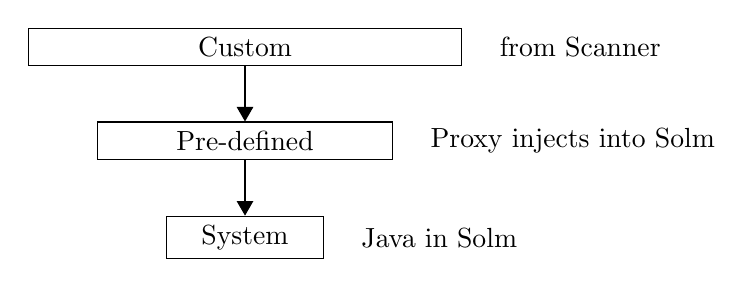
\begin{tikzpicture}[every node/.style={draw, text centered},
        every path/.style={-triangle 60, draw}]
        \node [text width=5em] (system) {System};
        \node [text width=10em, above=2em of system.north, anchor=south] (predefined) {Pre-defined};
        \node [text width=15em, above=2em of predefined.north, anchor=south] (custom) {Custom};
        \node [draw=none, right=1em of system] {Java in \type{Solm}};
        \node [draw=none, right=1em of predefined] {\type{Proxy} injects into \type{Solm}};
        \node [draw=none, right=1em of custom] {from \type{Scanner}};
        \path (custom) -- (predefined);
        \path (predefined) -- (system);
    \end{tikzpicture}

    \subsection{System Predicates}

        System predicates and formulas are ($x_i$ is a variable, $p_i$ is a predicate,
        $X_i$ is a set of variables):

        \begin{maths}
        $\type{true}$ & always true\\
        $\alpha(x_1, x_2, \dots, x_n): p.$ & declaration of a new predicate $\alpha$\\
        $\exists x (p)$ & existence quantifier \\
        $\forall x (p)$ & universal quantifier  \\
        $p_1 \vee p_2 \vee \dots \vee p_n$ & logical disjunction \\
        $p_1 \wedge p_2 \wedge \dots \wedge p_n$ & logical conjunction \\
        $p_1 \to p_2 \to \dots \to p_n$ & logical implication \\
        $x \in X$ & $x$ belongs to set $X$ \\
        $\neg p$ & predicate $p$ is false \\
        $x_1 = x_2$ & variable $x_1$ equals to variable $x_2$ \\
        $x_1 < x_2$ & variable $x_1$ is less than variable $x_2$ \\
        $\type{kind}(x_1, x_2)$ & $x_1$ is a variable of kind $x_2$ \\
        $\type{re}(x_1, x_2)$ & variable $x_1$ matches regular expression $x_2$\\
        $\type{ac}(x_1, x_2, x_3)$ & variable $x_1$ has access $x_3$ to variable $x_2$ \\
        \end{maths}

        A variable can be represented by an \textit{atom}, which starts with a single
        quotation mark (like in Lisp~\cite{graham93}), for example:

        $$\exists X (\forall x(x \in X \to x < \type{'5}) \wedge X = \type{'3})$$

        A variable can be represented by a \textit{set},
        which looks like:

        $$\exists x (x = \{y, \type{'5}\})$$

        Only declaration and quantifiers can declare a variable (create
        a new variable). All other predicates will report a fatal error
        if an undefined variable is passed to them.

        Predicates are realized in \type{Solm} as a collection of \emph{formulas}
        (classes inherited from \type{Formula}):

        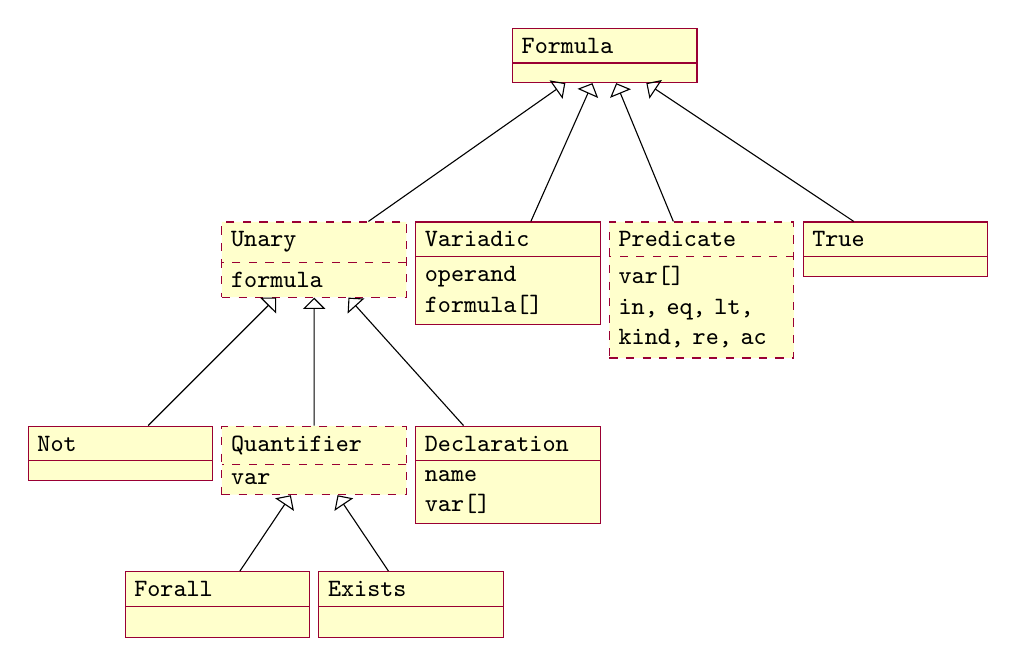
\begin{tikzpicture}[
            every node/.style={class},
            level 1/.style={level distance=6em, sibling distance=7em, open triangle 90-},
            level 2/.style={sibling distance=7em},
            ]
            \tikzstyle{class} = [text width=6em, font={\small\ttfamily}, fill=white, anchor=north,
                rectangle split, rectangle split parts=2,
                fill=rupBody, draw=rupBorder];
            \node {Formula\nodepart{second}}
                child {node [dashed] {Unary\nodepart{second} formula}
                    child {node {Not\nodepart{second}}}
                    child {node [dashed] {Quantifier\nodepart{second} var}
                        child [level distance=4em] {node {Forall}}
                        child [level distance=4em] {node {Exists}}
                    }
                    child {node {Declaration\nodepart{second} name\linebreak var[]}}
                }
                child {node {Variadic\nodepart{second} operand\linebreak formula[]}}
                child {node [dashed] {Predicate\nodepart{second} var[]
                    \linebreak
                    in, eq, lt, kind, re, ac}}
                child {node {True\nodepart{second}}}
            ;
        \end{tikzpicture}

        This structure is fixed and is not going to change. All other predicates
        are defined on top of these.

    \subsection{Pre-defined Predicates}

        Before the conversion is started \texttt{Proxy}
        injects into \texttt{Solm} a number of ``pre-defined
        predicates'', in order to enable other predicates in SOLM:

        \begin{maths}
        $\type{created}(x_1, x_2): \type{ac}(x_1, x_2, \type{'C}). $ \\
        $\type{read}(x_1, x_2): \type{ac}(x_1, x_2, \type{'R}). $ \\
        $\type{updated}(x_1, x_2): \type{ac}(x_1, x_2, \type{'U}). $ \\
        $\type{deleted}(x_1, x_2): \type{ac}(x_1, x_2, \type{'D}) \wedge \forall x (x \neq x_1). $ \\
        $\type{exception}(x): \exists x_2 (x_2 = x \wedge \type{kind}(x_2, \type{'ex}))$ \\
        $\type{throw}(x): \type{kind}(x, \type{'ex}) \wedge \neg \type{true}$ \\
        $\type{info}(x): \type{kind}(x_2, \type{'info}). $ \\
        $\type{silent}(x): \type{kind}(x_2, \type{'silent}). $ \\
        $\type{err}(x): \type{kind}(x_2, \type{'err}). $ \\
        $\type{number}(x): \type{kind}(x, \type{'number}) \wedge \type{re}(x, \type{'[0-9]+}).$ \\
        $\type{text}(x): \type{kind}(x, \type{'text}).$ \\
        $\type{SUD}(x): \type{kind}(x, \type{'actor}).$ \\
        \end{maths}

        Also math binary predicates:

        \begin{maths}
        $x_1 > x_2: \neg(x_1 < x_2) \wedge \neg(x_1 = x_2). $ \\
        $x_1 \geq x_2: \neg (x_1 < x_2). $ \\
        $x_1 \leq x_2: x_1 < x_2 \vee x_1 = x_2. $ \\
        $x_1 \neq x_2: \neg (x_1 = x_2). $ \\
        \end{maths}

    \subsection{Types to Predicates}

        Let's convert a type defined above to second order logic predicates.
        First, we define predicates for slots inside the type (a few examples):

        \begin{maths}
        $\type{User.photo}(x, p): \type{kind}(x, \type{'User}) \wedge \type{Photo}(p) \wedge$ \\
        $\quad \exists r (\type{kind}(r, \type{'User.email}) \wedge r = \{x, p\}). $ \\
        $\type{User.address.country}(x, p): \type{kind}(x, \type{'User}) \wedge \type{text}(p)$ \\
        $\quad \exists r (\type{kind}(r, \type{'User.address.country}) \wedge r = \{x, p\}). $ \\
        \end{maths}

        Then we create predicates for types ($\Pi_i$ is a set):

        \begin{maths}
        $\type{User}(x) :$ \\
        $\quad \type{kind}(x, \type{'User}) \bigwedge$ \\
        $\quad \exists \Pi_1 (\Pi_1 = \type{'1} \wedge \forall p(p \in \Pi_1 \to \type{User.email}(x, p)) \bigwedge$ \\
        $\quad \exists \Pi_2 (\Pi_2 \geq \type{'0} \wedge \forall p(p \in \Pi_2 \to \type{User.photo}(x, p)) \bigwedge$ \\
        $\quad \exists \Pi_3 (\Pi_3 < \type{'2} \wedge \forall p(p \in \Pi_3 \to \type{User.manager}(x, p)) \bigwedge $ \\
        $\quad \exists \Pi_4 (\Pi_4 = \type{'1} \wedge \forall p(p \in \Pi_4 \to \type{User.address.city}(x, p)) \bigwedge $ \\
        $\quad \exists \Pi_5 (\Pi_5 = \type{'1} \wedge \forall p(p \in \Pi_5 \to \type{User.address.country}(x, p)). $ \\
        \end{maths}

    \subsection{Use Case to Predicate}

        Every use case is a predicate, $\type{UC}_1(x) = \type{true}$ means that the user
        successfully extended his photo album:

        \begin{maths}
        $\type{UC}_1(x) : $ \\
        $\quad \type{User}(x) \bigwedge$ \\
        $\quad \exists s (\type{SUD}(s)) \bigwedge$ \\
        $\quad \exists \Pi(\forall p (p \in \Pi \to \type{User.photo}(x, p))) \bigwedge$ \\
        $\quad \neg (\Pi > 5) \bigvee $ \\
        $\quad ($ \\
        $\quad\quad \type{info}(\type{'If number of photos of the user is greater than 5})\bigwedge$ \\
        $\quad\quad \exists y(y \in \Pi) \bigwedge$ \\
        $\quad\quad \type{deleted}(y, x) \wedge \type{info}(\type{'The user deletes photo of himself})$ \\
        $\quad ) \bigwedge$ \\
        $\quad \exists p(p \in \Pi) \bigwedge$ \\
        $\quad \type{created}(p, x) \wedge \type{info}(\type{'The user creates photo of himself (the photo)})\bigwedge$ \\
        $\quad \type{UC}_2(p) \wedge \type{info}(\type{'We validate the photo immediately}) \vee$ \\
        $\quad ($ \\
        $\quad\quad \type{exception}(\type{'file format is not valid}) \bigwedge$ \\
        $\quad\quad \type{deleted}(p, s) \wedge \type{info}(\type{'We delete the photo})\bigwedge$ \\
        $\quad\quad \type{throw}(\type{'only PNG images are accepted})$ \\
        $\quad ) \bigwedge$ \\
        $\quad \type{silent}(\type{We protocol the operation in backlog})\bigwedge$ \\
        $\quad \type{read}(p, x)\wedge \type{info}(\type{'The user reads the photo})$ \\
        \end{maths}





\section{Predicates to Snapshots}
\label{sec:to-data}

    Every formula produces a number of ``fact paths''. Every fact path
    is a vector of ``facts'', and every fact is either a positive or negative:

    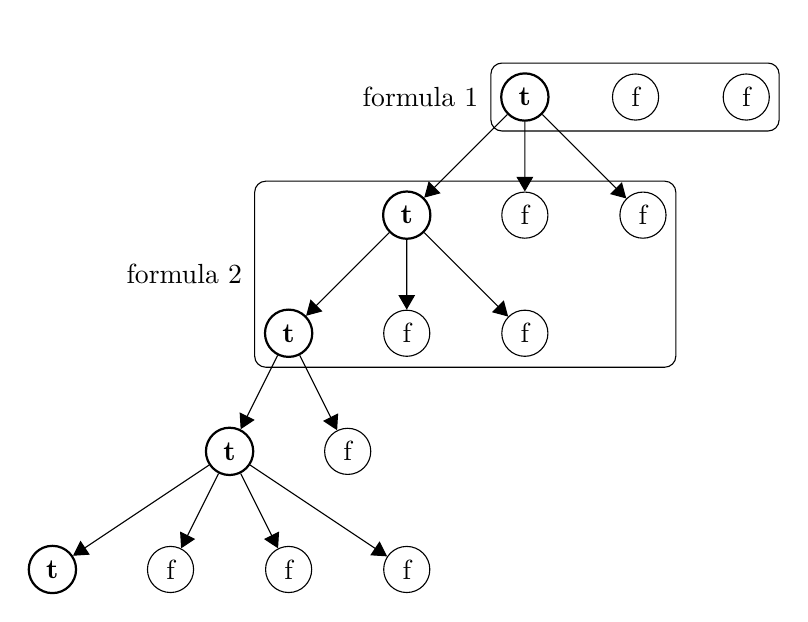
\begin{tikzpicture}[
        node distance=4em,
        every node/.style={circle, draw},
        level 1/.style={},
        level 2/.style={},
        -triangle 60
        ]
        \tikzstyle{true} = [thick, font=\bfseries];
        \node[true] (t1) {t}
            child {node[true] (t2-1) {t}
                child {node[true] (t2-1-1) {t}
                    child {node[true] {t}
                        child {node[true] {t}}
                        child {node {f}}
                        child {node {f}}
                        child {node {f}}
                    }
                    child {node {f}}
                }
                child {node (t2-1-2) {f}}
                child {node (t2-1-3) {f}}
            }
            child {node (t2-2) {f}}
            child {node (t2-3) {f}}
        ;
        \node [right of=t1] (t2) {f};
        \node [right of=t2] (t3) {f};

        \node [draw=black, rectangle, rounded corners, fit=(t1) (t2) (t3)] (f1) {};
            \node [draw=none, anchor=east] at (f1.west) {formula 1};

        \node [draw=black, rectangle, rounded corners, fit=(t2-1) (t2-1-1) (t2-1-2) (t2-1-3) (t2-2) (t2-3)] (f2) {};
            \node [draw=none, anchor=east] at (f2.west) {formula 2};
    \end{tikzpicture}

    Every fact includes a ``snapshot'' of persistent data. Snapshot includes:
    objects. Every object
    has a name, value, type,
    and may have a number of changes made by other objects:

    \begin{lstlisting}[language=Java]
class Object {
    int id; // could be zero
    string name; // could be empty
    string type; // mandatory
    Value* value;
    vector<AclRule> rules;
};
class Value {};
    class ValueString : public Value {
        string value;
    };
    class ValueSet : public Value {
        vector<int> ids;
    };
    class ValueAssociation : public Value,
        public pair<AssociationMember, AssociationMember> {};
        class AssociationMember {};
            class AssociationMemberId : public AssociationMember {
                int id;
            };
            class AssociationMemberName : public AssociationMember {
                string name;
            };
class AclRule {
    enum {CREATE, READ, UPDATE, DELETE} operation;
    int id;
};
vector<Object> snapshot;
\end{lstlisting}

    Consider this example:

    \def\chng#1{\colorbox{lightgray}{#1}}
    \begin{tabular}[t]{l|lllll}
        SOLM formula & \multicolumn{5}{l}{Snapshots} \\
        & Name & Type & ID & Value & ACL Rules \\
        \hline

        $\type{UC}_1(x) : $ \\
        $\quad \type{User}(x) \to$
            & \chng{$x$} & \chng{\texttt{User}} & \chng{\texttt{1}} \\

        \hline
        $\quad \exists \Pi(\type{User.photo}(x, \Pi)) \to$
            & $x$ & \texttt{User} & \texttt{1} \\
            & \chng{$\Pi$} & \chng{\texttt{Photo}} & & \chng{\texttt{[?]}} \\
            &  & \chng{\texttt{User.photo}} & & \chng{\texttt{1:$\Pi$}} \\

        \hline
        $\quad ($ \\
        $\quad\quad |\Pi| > 5 \to$
            & $x$ & \texttt{User} & \texttt{1} \\
            & $\Pi$ & \texttt{Photo} & & \texttt{[\chng{2}]} \\
            &  & \chng{\texttt{Photo}} & \chng{\texttt{2}} \\
            & & \texttt{User.photo} & \texttt{\chng{3}} & \chng{\texttt{1:2}} \\

        \hline
        $\quad\quad \exists y(y \in \Pi) \to$ \\
        $\quad\quad \type{deleted}(y) $ \\
        $\quad ) \to$
            & \multicolumn{4}{l}{\textit{skipped}} \\

        \hline
        $\quad \exists p(p \in \Pi) \to$
            & $x$ & \texttt{User} & \texttt{1} \\
            & $\Pi$ & \texttt{Photo} & & \texttt{[2]} \\
            & \chng{$p$} & \texttt{Photo} & \texttt{2} \\
            &  & \texttt{User.photo} & \texttt{3} & \texttt{1:2} \\

        \hline
        $\quad \type{created}(p, x) \to$
            & $x$ & \texttt{User} & \texttt{1} \\
            & $\Pi$ & \texttt{Photo} & & \texttt{[2\chng{,4}]} \\
            & \chng{---} & \texttt{Photo} & \texttt{2} \\
            & \chng{$p$} & \chng{\texttt{Photo}} & \chng{\texttt{4}} & & \chng{\texttt{CREATE:1}} \\
            & & \texttt{User.photo} & & \texttt{1:2} \\
            & & \chng{\texttt{User.photo}} & \chng{\texttt{5}} & \chng{\texttt{1:4}} \\

        \hline
        $\quad \type{UC}_2(p) \vee$ \\
        $\quad ($ \\
        $\quad\quad \type{exception}(\mbox{``file format...''}) \to$ \\
        $\quad\quad \type{deleted}(p) \to$ \\
        $\quad\quad \type{throw}(\mbox{``only PNG...''})$ \\
        $\quad ) \to$
            & \multicolumn{5}{l}{\textit{skipped}} \\

        \hline
        $\quad \type{silent}(\mbox{``We protocol...''})$ \\
        $\quad \type{read}(p, x) $
            & $x$ & \texttt{User} & \texttt{1} \\
            & $\Pi$ & \texttt{Photo} & & \texttt{[2,4]} \\
            &  & \texttt{Photo} & \texttt{2} \\
            & $p$ & \texttt{Photo} & \texttt{4} & & \texttt{CREATE:1}\chng{,} \\
            &     &                &            & & \chng{\texttt{READ:1}} \\
            & & \texttt{User.photo} & & \texttt{1:2} \\
            & & \texttt{User.photo} & & \texttt{1:4} \\
            & & \chng{\texttt{silent}} & \chng{\texttt{6}} &
                \chng{\parbox[t]{5em}{\raggedright``We protocol...''}} \\

    \end{tabular}





\section{Command Line Interface}
\label{sec:front}

    CLI is a collection of components. Every component gets
    an associative array of configuration parameters
    and returns an XML element. The element is named \texttt{<report>}
    and has attributes equivalent to the configuration
    params provided.

    \texttt{main()} returns an XML document that integrates
    all reports retrieved:

    \begin{lstlisting}[language=XML]
<?xml version="1.0" ?>
<rqdql>
  <errors>
    <report>
      <error line="23">This is an error</error>
    </report>
  </errors>
  <metrics>
    <report>
      <ambiguity>0.765</ambiguity>
    </report>
  </metrics>
  <uml>
    <report uc="UC6.5">
      <uml><[CDATA[....]]></uml>
    </report>
  </uml>
</rqdql>
    \end{lstlisting}

    The script shall be called from command line like this:

    \begin{lstlisting}[language=bash]
$ java -jar rqdql-bin.jar errors uml:uc=UC6.5 metrics < myscope.txt
    \end{lstlisting}

    Possible reports are:

    \begin{itemize}
        \item \texttt{errors}: full list of errors
        \item \texttt{metrics}: full analysis of the scope ambiguity, size, intensity, etc.
        \item \texttt{links}: report links between objects (line to line)
        \item \texttt{uml:uc=UC5,type=ActorUser,...}: description of types and use cases in UML
        \item \texttt{svg:uc=UC5,type=ActorUser,...}: description of types and use cases in SVG
        \item \texttt{tc:uc=UC5,...}: Test Cases for the given UC-s (or all)
    \end{itemize}





\section{Test Cases}
\label{sec:test-cases}

    We optimize vectors of snapshots, in order
    to produce the smallest collection.
    Then, we convert a vector of snapshots into MOF meta-model.
    The process looks like this:

    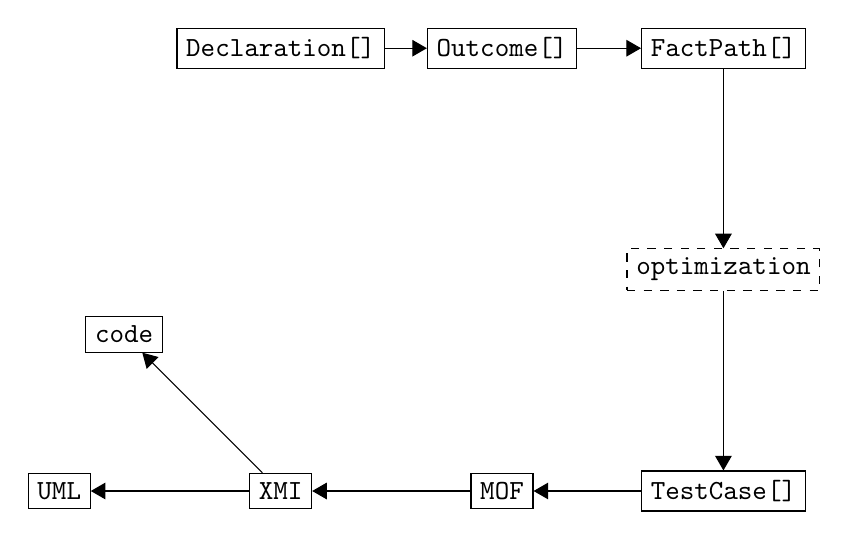
\begin{tikzpicture}[node distance=8em, -triangle 60, font=\ttfamily]
        \node [draw] (declarations) {Declaration[]};
        \node [draw, right of=declarations] (outcomes) {Outcome[]};
        \node [draw, right of=outcomes] (paths) {FactPath[]};
        \node [draw, dashed, below of=paths] (optimization) {optimization};
        \node [draw, below of=optimization] (tcs) {TestCase[]};
        \node [draw, left of=tcs] (mof) {MOF};
        \node [draw, left of=mof] (xmi) {XMI};
        \node [draw, left of=xmi] (uml) {UML};
        \node [draw, above left of=xmi] (code) {code};

        \draw (declarations) -- (outcomes);
        \draw (outcomes) -- (paths);
        \draw (paths) -- (optimization);
        \draw (optimization) -- (tcs);
        \draw (tcs) -- (mof);
        \draw (mof) -- (xmi);
        \draw (xmi) -- (uml);
        \draw (xmi) -- (code);
    \end{tikzpicture}





\section{Architecture and Design}
\label{sec:design}

    This section is under construction and the material
    you find below is just a preliminary draft pictures
    to keep me focused on the subject. Consider them as
    working drafts...

    \begin{tikzpicture}
        [node distance=8em]
        \node [draw] (yacc) {YACC};
        \node [draw, right of=yacc] (brokers) {C++ brokers};
        \node [draw, right of=brokers] (proxy) {Proxy};
        \node [draw, right of=proxy] (solm) {Solm};

        \node [draw, below of=proxy] (logger) {Logger};
        \node [draw, right of=logger] (front) {Front};
        \node [draw, right of=front] (main) {\texttt{main()}};
        \node [draw, below of=main] (plugin) {RqdqlPlugin};

        \draw [->] (yacc) -- (brokers);
        \draw [->] (brokers) -- (proxy);
        \draw [->] (proxy) -- (solm);
        \draw [->] (main) -- (front);
        \draw [->] (front) -- (logger);
        \draw [->] (front) -- (solm);
        \draw [->] (plugin) -- (main);

        \draw [dashed, ->] (yacc) -- (logger);
        \draw [dashed, ->] (brokers) -- (logger);
        \draw [dashed, ->] (proxy) -- (logger);
        \draw [dashed, ->] (solm) -- (logger);
    \end{tikzpicture}



%\bibliography{?}{}
%\bibliographystyle{plain}

\end{document}
